% =============================================================================
% WestQuant Paper Template
% =============================================================================
% Paper: Representation as a Variable: Cross-Framework Variance
%        Decomposition for Quantum Compilation
%
% Compile with: tectonic main.tex  (or pdflatex/xelatex)
%
% Author: David Vesterlund, WestQuant Open Source
% Contact: david@vesterlundventures.se
% =============================================================================

\documentclass[11pt,a4paper]{article}

% --- Page geometry ---
\usepackage[margin=2.5cm]{geometry}

% --- Math ---
\usepackage{amsmath,amssymb,amsthm}

% --- Figures and tables ---
\usepackage{graphicx}
\usepackage{booktabs}
\usepackage{tabularx}
\usepackage{multirow}
\usepackage{float}
\usepackage{array}
\usepackage{longtable}
\usepackage{subcaption}

% --- Text and layout ---
\usepackage{xcolor}
\usepackage{enumitem}
\usepackage{caption}
\usepackage{titlesec}
\usepackage{fancyhdr}
\usepackage{wrapfig}

% --- References and links ---
\usepackage[numbers,sort&compress]{natbib}
\usepackage{hyperref}
\usepackage{url}

\hypersetup{
    colorlinks=true,
    linkcolor=blue!70!black,
    citecolor=blue!70!black,
    urlcolor=blue!70!black
}

% --- Section formatting ---
\titleformat{\section}{\large\bfseries}{\thesection}{1em}{}
\titleformat{\subsection}{\normalsize\bfseries}{\thesubsection}{1em}{}

% --- Headers ---
\pagestyle{fancy}
\fancyhf{}
\fancyhead[L]{\small\itshape Representation as a Variable}
\fancyhead[R]{\small\thepage}
\renewcommand{\headrulewidth}{0.4pt}

% =============================================================================
% TITLE AND AUTHOR
% =============================================================================

\title{\Large\textbf{Representation as a Variable: Cross-Framework Variance Decomposition for Quantum Compilation}}
\author{%
  David Vesterlund \\
  Industrial Research at Vesterlund Ventures \\
  WestQuant Open Source Project \\
  \texttt{david@vesterlundventures.se}%
}
\date{}

\begin{document}

\maketitle
\thispagestyle{empty}

% =============================================================================
% ABSTRACT
% =============================================================================

\begin{abstract}
\noindent
\textbf{Key finding:} The framework $\times$ algorithm interaction explains 32--42\% of circuit depth variance across 6--12 qubit circuits---exceeding the framework main effect (10--14\%) and approaching the algorithm main effect (23--34\%). No single compilation framework is universally optimal; the best framework depends on the algorithm, and representation search within a framework explains up to 78\% of depth variance at 12 qubits.

\medskip
\noindent
A quantum algorithm does not determine a unique compiled circuit. The choice of compilation framework, configuration within that framework, and the interaction between the two jointly determine the final circuit depth, gate count, and two-qubit gate count. We treat this representation choice as an optimization variable and ask: how much of compilation quality variance comes from the framework, from the configuration, and from their interaction?

We conduct a large-scale empirical study across four quantum compilation frameworks (Qiskit, PyTKET, PennyLane, Cirq), six benchmark algorithms (QFT, Grover, QPE, GHZ, Bernstein--Vazirani, and a superposition circuit), four circuit sizes (6, 8, 10, 12 qubits), and three replicates per cell, yielding 4{,}608 observations. We apply a two-factor variance decomposition (algorithm $\times$ framework) and a within-framework decomposition (algorithm vs.\ configuration).

We find three results. First, the framework $\times$ algorithm interaction explains 32--42\% of circuit depth variance (mean 39\%), exceeding the framework main effect (mean 12\%) and approaching the algorithm main effect (mean 29\%). No single framework dominates for all algorithms. Second, configuration choice within a single framework explains up to 78\% of depth variance at 12 qubits, and this fraction grows with circuit size. Third, the four frameworks expose structurally different representation search spaces---ranging from 6 to 128 configurations across different compilation dimensions---meaning the ``representation space'' is framework-defined, not universal.

These findings support the thesis that representation is a genuine optimization variable: the choice of how to compile a quantum algorithm matters as much as the choice of algorithm itself, and its importance grows with circuit scale.
\end{abstract}

\vspace{0.5em}
\noindent\textbf{Keywords:} quantum compilation, representation search, variance decomposition, multi-framework benchmarking, NISQ, combinatorial optimization

% =============================================================================
% HEADLINE FIGURE
% =============================================================================

\begin{figure}[H]
\centering
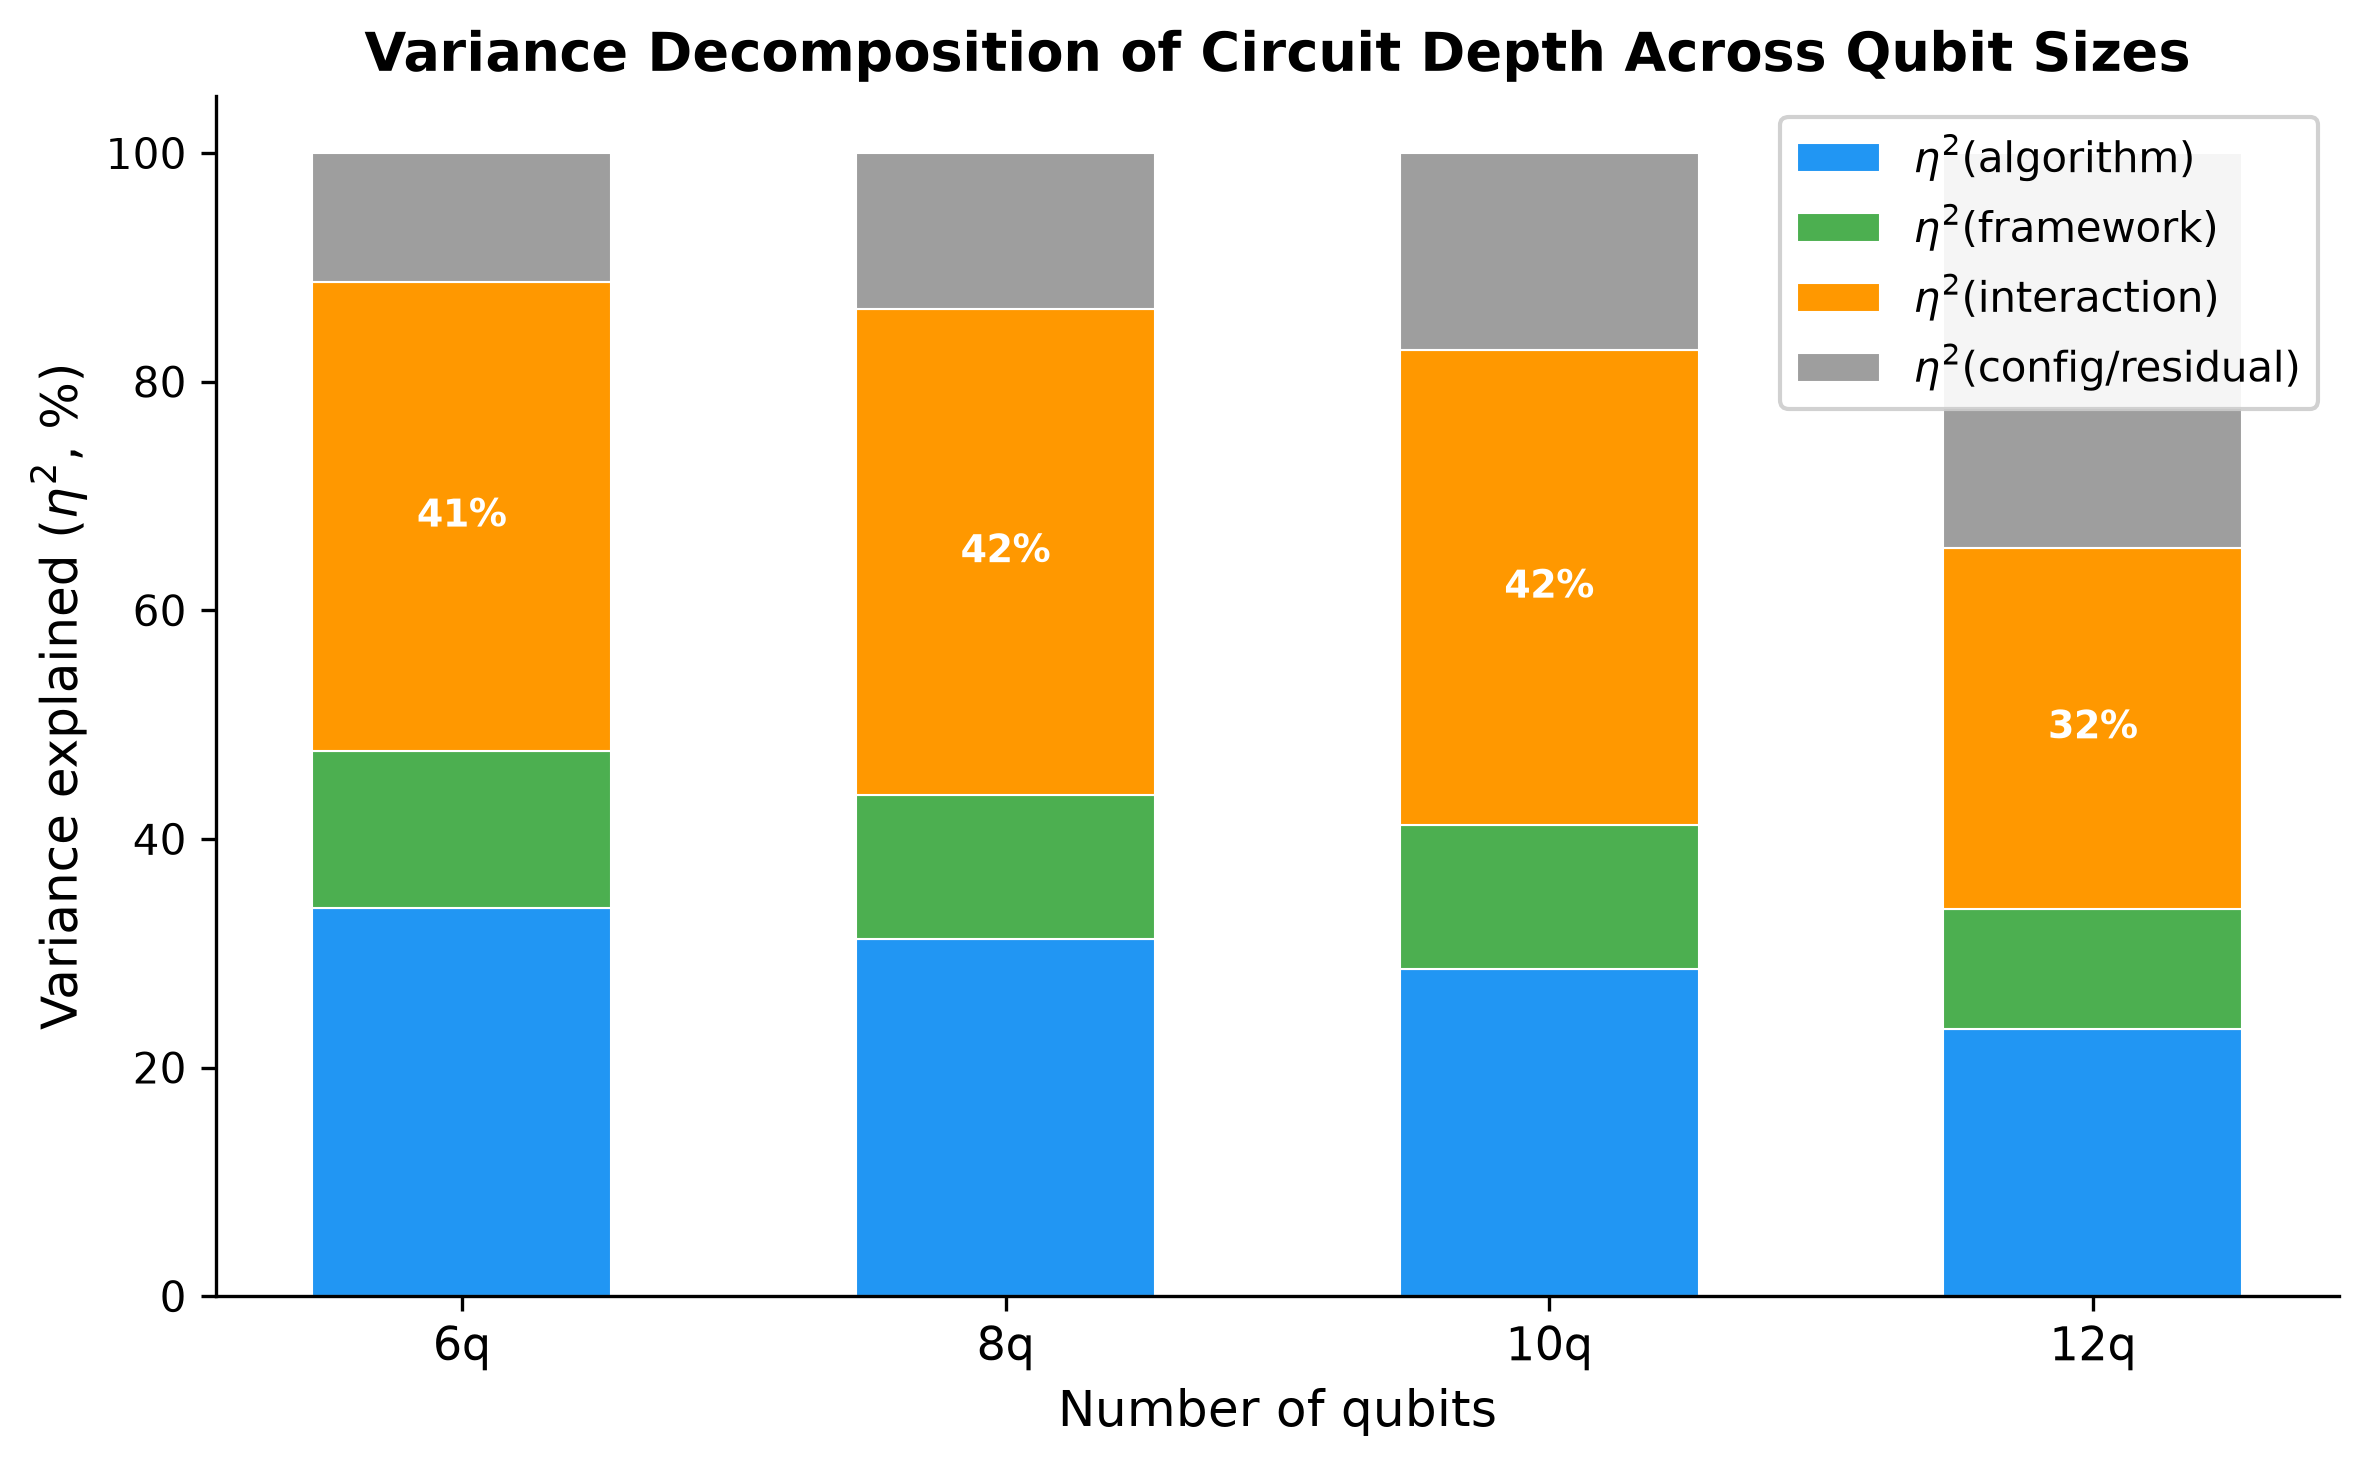
\includegraphics[width=0.85\textwidth]{../figures/fig1_variance_decomposition.png}
\caption{\textbf{Variance decomposition of circuit depth across qubit sizes.} Each bar shows the proportion of depth variance explained by algorithm identity ($\eta^2_{\text{algorithm}}$), framework choice ($\eta^2_{\text{framework}}$), their interaction ($\eta^2_{\text{interaction}}$), and residual configuration variance ($\eta^2_{\text{residual}}$). The interaction effect (orange) is the dominant factor at 6--10 qubits (41--42\%), demonstrating that no single framework is universally optimal. At 12 qubits, the residual (grey) grows to 35\%, indicating that within-framework configuration choice becomes the primary lever at scale.}
\label{fig:variance_decomposition}
\end{figure}

\newpage

% =============================================================================
% 1. INTRODUCTION
% =============================================================================

\section{Introduction}

\subsection{The representation problem}

A quantum algorithm is typically specified as an abstract circuit over idealized gates. Before execution on hardware, this circuit must be compiled: mapped to a target gate set, routed to a physical connectivity graph, and optimized for depth and fidelity. This compilation pipeline is not unique. Different compilation frameworks (Qiskit~\cite{ref1}, PyTKET~\cite{ref2}, PennyLane~\cite{ref3}, Cirq~\cite{ref4}) implement different passes, heuristics, and gate decompositions. Within each framework, different configuration choices (layout method, routing strategy, optimization level, gate set) produce different compiled circuits from the same input.

The conventional approach treats compilation as a fixed transformation: the user selects a framework, accepts its default configuration, and executes the resulting circuit. This approach implicitly assumes that the representation---the specific compiled circuit---is determined by the algorithm and the framework, with configuration providing minor adjustments.

We challenge this assumption. We treat the representation itself as an optimization variable and ask how much it matters. Specifically:

\begin{itemize}[noitemsep]
\item \textbf{RQ1:} How much of compilation quality variance is explained by the framework choice, the configuration choice within a framework, and their interaction?
\item \textbf{RQ2:} Does the importance of representation choice change with circuit scale?
\item \textbf{RQ3:} Do different frameworks expose comparable representation search spaces, or are they structurally different?
\end{itemize}

\subsection{Contributions}

This paper makes the following contributions:

\begin{enumerate}[noitemsep]
\item A large-scale cross-framework benchmark of 4{,}608 compilation observations across 4 frameworks, 6 algorithms, 4 circuit sizes, and 3 replicates, with all data publicly available.
\item A two-factor variance decomposition showing that the framework $\times$ algorithm interaction explains 32--42\% of depth variance, demonstrating that no single framework is universally optimal.
\item A within-framework decomposition showing that configuration choice explains up to 78\% of depth variance at 12 qubits, with this fraction growing with circuit scale.
\item A structural comparison of framework search spaces, showing that the four frameworks expose fundamentally different representation dimensions, not merely different parameterizations of the same space.
\item Evidence that representation search yields substantial improvements: the best configuration reduces depth by a median of 29\% and a maximum of 99\% relative to the mean configuration, with 47\% of cells showing improvements exceeding 30\%.
\end{enumerate}

\subsection{Related work}

Cross-framework benchmarking of quantum compilers has been explored in the QED-C benchmark suite~\cite{ref5} and in individual comparisons of Qiskit vs.\ Cirq~\cite{ref6} or PyTKET vs.\ Qiskit~\cite{ref7}. These studies compare frameworks at their default settings and report aggregate performance metrics. They do not decompose variance into framework, configuration, and interaction effects, and they do not treat representation as a search variable.

Multi-objective optimization in quantum compilation has been studied for specific frameworks, including Pareto-optimal transpilation in Qiskit~\cite{ref8} and depth-fidelity trade-offs in PyTKET~\cite{ref9}. These approaches optimize within a single framework and do not compare across frameworks.

The idea of treating compilation as a search problem has been explored in compiler autotuning for classical systems~\cite{ref10} and in ML-guided quantum compilation~\cite{ref11}. Our contribution is to formalize the representation search problem across frameworks and to quantify the variance decomposition that justifies it.

The WestQuant open-source ecosystem~\cite{ref12} provides the tooling for this study: a unified search interface across frameworks, provenance tracking via representation graphs, structured training record export in the WQDF (WestQuant Dataset Format), and benchmark circuit generators for cross-framework comparison.

% =============================================================================
% 2. METHODS
% =============================================================================

\section{Methods}

\subsection{Frameworks}

We evaluate four quantum compilation frameworks, each exposing a different representation search space:

\textbf{Qiskit} (v2.5.2, via \texttt{westquant-qiskit} v0.1.0a4) searches the compiler configuration space with four stages: optimization level (0--3), layout method (trivial, dense, sabre, default), routing method (basic, sabre, lookahead, default), and translation method (translator, synthesis). The full grid contains 128 configurations; we test a 32-configuration subset (4 $\times$ 2 $\times$ 2 $\times$ 1 with seed fixed) using both deterministic grid search and sequential beam search (beam width 3).

\textbf{PyTKET} (v2.18.4, via \texttt{westquant-pytket} v0.1.0a2) searches the compilation pass selection space with four stages: optimization (none, redundancies, peephole, synthesise), placement (none, naive, graph), routing (none, routing, aas), and rebase (none, tket, synthesise). The full grid contains 108 configurations; we explore via sequential beam search (beam width 3), evaluating 32 states per run.

\textbf{PennyLane} (v0.45.1, via \texttt{westquant-pennylane} v0.1.0a1) searches the gate-level transform space with four stages: commute (none, commute\_right, commute\_left), cancel (none, cancel\_inverses), merge (none, merge\_rotations), and cleanup (none, remove\_barrier). The full grid contains 24 configurations; we explore via sequential beam search (beam width 3), evaluating 22 states per run.

\textbf{Cirq} (v1.7.0, via \texttt{westquant-bridges} v0.1.0a2) searches the gate set and pass count space with two stages: gate set (CZ, sqrt-iSWAP) and max passes (1, 2, 4). The full grid contains 6 configurations; we explore via sequential beam search (beam width 3), evaluating 9 states per run.

Table~\ref{tab:search_spaces} summarizes the search spaces.

\begin{table}[H]
\centering
\caption{Representation search spaces across frameworks.}
\label{tab:search_spaces}
\begin{tabular}{lccccc}
\toprule
Framework & Stages & Configs (avail.) & Configs (tested) & Search type & Nature \\
\midrule
Qiskit & 4 & 128 & 32 & Grid + beam & Compiler configuration \\
PyTKET & 4 & 108 & 32 & Sequential beam & Pass selection \\
PennyLane & 4 & 24 & 22 & Sequential beam & Gate-level transforms \\
Cirq & 2 & 6 & 9 & Sequential beam & Gate set + passes \\
\bottomrule
\end{tabular}
\end{table}

A key observation is that these search spaces are structurally different, not merely different parameterizations of the same space. Qiskit and PyTKET search compiler configuration space (which passes to apply). PennyLane searches gate-level transform space (which gate-level rewrites to apply). Cirq searches gate set and pass count (which target gate set and how many optimization passes). The dimensionality ranges from 2 (Cirq) to 4 (Qiskit, PyTKET, PennyLane), and the number of available configurations ranges from 6 (Cirq) to 128 (Qiskit).

\subsection{Algorithms}

We evaluate six quantum algorithms spanning different circuit structures. Benchmark circuits for QFT, Grover, and GHZ are generated using the \texttt{westquant-bridges} benchmark generators, which produce framework-native circuits for Qiskit and Cirq. QPE, BV, and Superposition use custom generators:

\begin{itemize}[noitemsep]
\item \textbf{QFT} (Quantum Fourier Transform): structured, periodic, depth grows $O(n^2)$. Tests routing on nearest-neighbor architectures.
\item \textbf{Grover}: unstructured search with multi-controlled oracle. Tests decomposition of multi-controlled gates and oracle structure.
\item \textbf{QPE} (Quantum Phase Estimation): structured, combines controlled-phase with inverse QFT. Tests composition of subroutines.
\item \textbf{GHZ}: entanglement benchmark with minimal circuit (H + CNOT chain). Tests simple chain routing.
\item \textbf{BV} (Bernstein--Vazirani): oracle-based, should compile to near-zero depth. Tests oracle pattern recognition.
\item \textbf{Superposition}: uniform superposition with light entanglement. Tests basic compilation.
\end{itemize}

All algorithms are generated in each framework's native circuit format to avoid conversion artifacts.

\subsection{Experimental design}

We use a factorial design:

\begin{itemize}[noitemsep]
\item \textbf{Qubit sizes:} 6, 8, 10, 12
\item \textbf{Algorithms:} QFT, Grover, QPE, GHZ, BV, Superposition
\item \textbf{Frameworks:} Qiskit, PyTKET, PennyLane, Cirq
\item \textbf{Replicates:} 3 (seeds 42, 43, 44)
\end{itemize}

Each cell (algorithm $\times$ framework $\times$ qubit size $\times$ replicate) produces multiple observations corresponding to different configurations explored by the search. The total dataset comprises 4{,}608 observations.

All experiments use a linear (nearest-neighbor) coupling map: $[(0,1), (1,2), \ldots, (n-2, n-1)]$ for $n$ qubits. This is a restrictive topology that forces routing, making the representation choice more impactful.

\subsection{Metrics}

We record three compilation metrics for each observation:

\begin{itemize}[noitemsep]
\item \textbf{Depth:} circuit depth (number of time steps)
\item \textbf{Size:} total gate count
\item \textbf{Two-qubit gates:} count of two-qubit operations (CNOT, CZ, etc.)
\end{itemize}

\subsection{Variance decomposition}

We apply a two-factor ANOVA-style variance decomposition:

$$Y_{ijk} = \mu + \alpha_i + \beta_j + (\alpha\beta)_{ij} + \epsilon_{ijk}$$

where $Y_{ijk}$ is the metric value, $\alpha_i$ is the algorithm effect, $\beta_j$ is the framework effect, $(\alpha\beta)_{ij}$ is the interaction, and $\epsilon_{ijk}$ is the residual (within-cell variance, corresponding to configuration choice and stochasticity).

We compute effect sizes as eta-squared:

$$\eta^2_A = \frac{SS_A}{SS_{\text{total}}}, \quad \eta^2_B = \frac{SS_B}{SS_{\text{total}}}, \quad \eta^2_{AB} = \frac{SS_{AB}}{SS_{\text{total}}}, \quad \eta^2_{\text{res}} = \frac{SS_{\text{res}}}{SS_{\text{total}}}$$

We also perform a within-framework decomposition for each framework, partitioning depth variance into algorithm effect and configuration effect (residual within framework).

% =============================================================================
% 3. RESULTS
% =============================================================================

\section{Results}

\subsection{Two-factor variance decomposition}

Table~\ref{tab:variance_depth} shows the variance decomposition for circuit depth at each qubit size.

\begin{table}[H]
\centering
\caption{Variance decomposition for circuit depth ($\eta^2$, \%)}
\label{tab:variance_depth}
\begin{tabular}{cccccc}
\toprule
Qubits & $\eta^2$(algorithm) & $\eta^2$(framework) & $\eta^2$(interaction) & $\eta^2$(residual) & $n$ \\
\midrule
6  & 34.0 & 13.7 & \textbf{41.0} & 11.3 & 1{,}152 \\
8  & 31.2 & 12.6 & \textbf{42.5} & 13.7 & 1{,}152 \\
10 & 28.6 & 12.6 & \textbf{41.6} & 17.2 & 1{,}152 \\
12 & 23.4 & 10.5 & \textbf{31.6} & 34.5 & 1{,}152 \\
\bottomrule
\end{tabular}
\end{table}

The framework $\times$ algorithm interaction is the dominant effect at 6--10 qubits, explaining 41--42\% of depth variance. This means the best framework depends on the algorithm: no single framework is universally optimal. At 12 qubits, the interaction decreases to 32\% while the residual (configuration choice within cells) grows to 35\%, indicating that at larger scales, within-framework configuration becomes an increasingly important lever.

Table~\ref{tab:variance_tqg} shows the same decomposition for two-qubit gate count.

\begin{table}[H]
\centering
\caption{Variance decomposition for two-qubit gate count ($\eta^2$, \%)}
\label{tab:variance_tqg}
\begin{tabular}{cccccc}
\toprule
Qubits & $\eta^2$(algorithm) & $\eta^2$(framework) & $\eta^2$(interaction) & $\eta^2$(residual) & $n$ \\
\midrule
6  & 66.5 & 16.9 & 19.5 & 0.0 & 1{,}041 \\
8  & 61.7 & 16.7 & 21.5 & 0.1 & 1{,}041 \\
10 & 58.5 & 17.2 & 22.7 & 1.6 & 1{,}041 \\
12 & 49.9 & 15.4 & 20.3 & 14.4 & 1{,}041 \\
\bottomrule
\end{tabular}
\end{table}

For two-qubit gates, the algorithm main effect dominates (50--67\%), but the interaction remains substantial (19--23\%) and stable across scales.

\subsection{Within-framework configuration variance}

Table~\ref{tab:within_framework} shows the within-framework decomposition: for each framework, how much of depth variance comes from configuration choice (as opposed to algorithm identity)?

\begin{table}[H]
\centering
\caption{Within-framework configuration variance ($\eta^2$ for configuration, \%)}
\label{tab:within_framework}
\begin{tabular}{lccccc}
\toprule
Framework & 6q & 8q & 10q & 12q & Trend \\
\midrule
PyTKET    & 54.8 & 60.6 & 72.0 & \textbf{77.8} & Growing \\
Qiskit    & 11.9 & 17.9 & 23.7 & \textbf{45.2} & Growing rapidly \\
PennyLane & 33.4 & 43.1 & 46.0 & \textbf{46.9} & Growing \\
Cirq      & 11.0 & 11.1 & 11.5 & \textbf{11.6} & Stable \\
\bottomrule
\end{tabular}
\end{table}

Three of four frameworks show increasing configuration variance with scale. For PyTKET at 12 qubits, 78\% of depth variance comes from configuration choice---more than from algorithm identity. For Qiskit, the growth is most dramatic: from 12\% at 6 qubits to 45\% at 12 qubits.

Figure~\ref{fig:config_variance} visualizes this growth trend.

\begin{figure}[H]
\centering
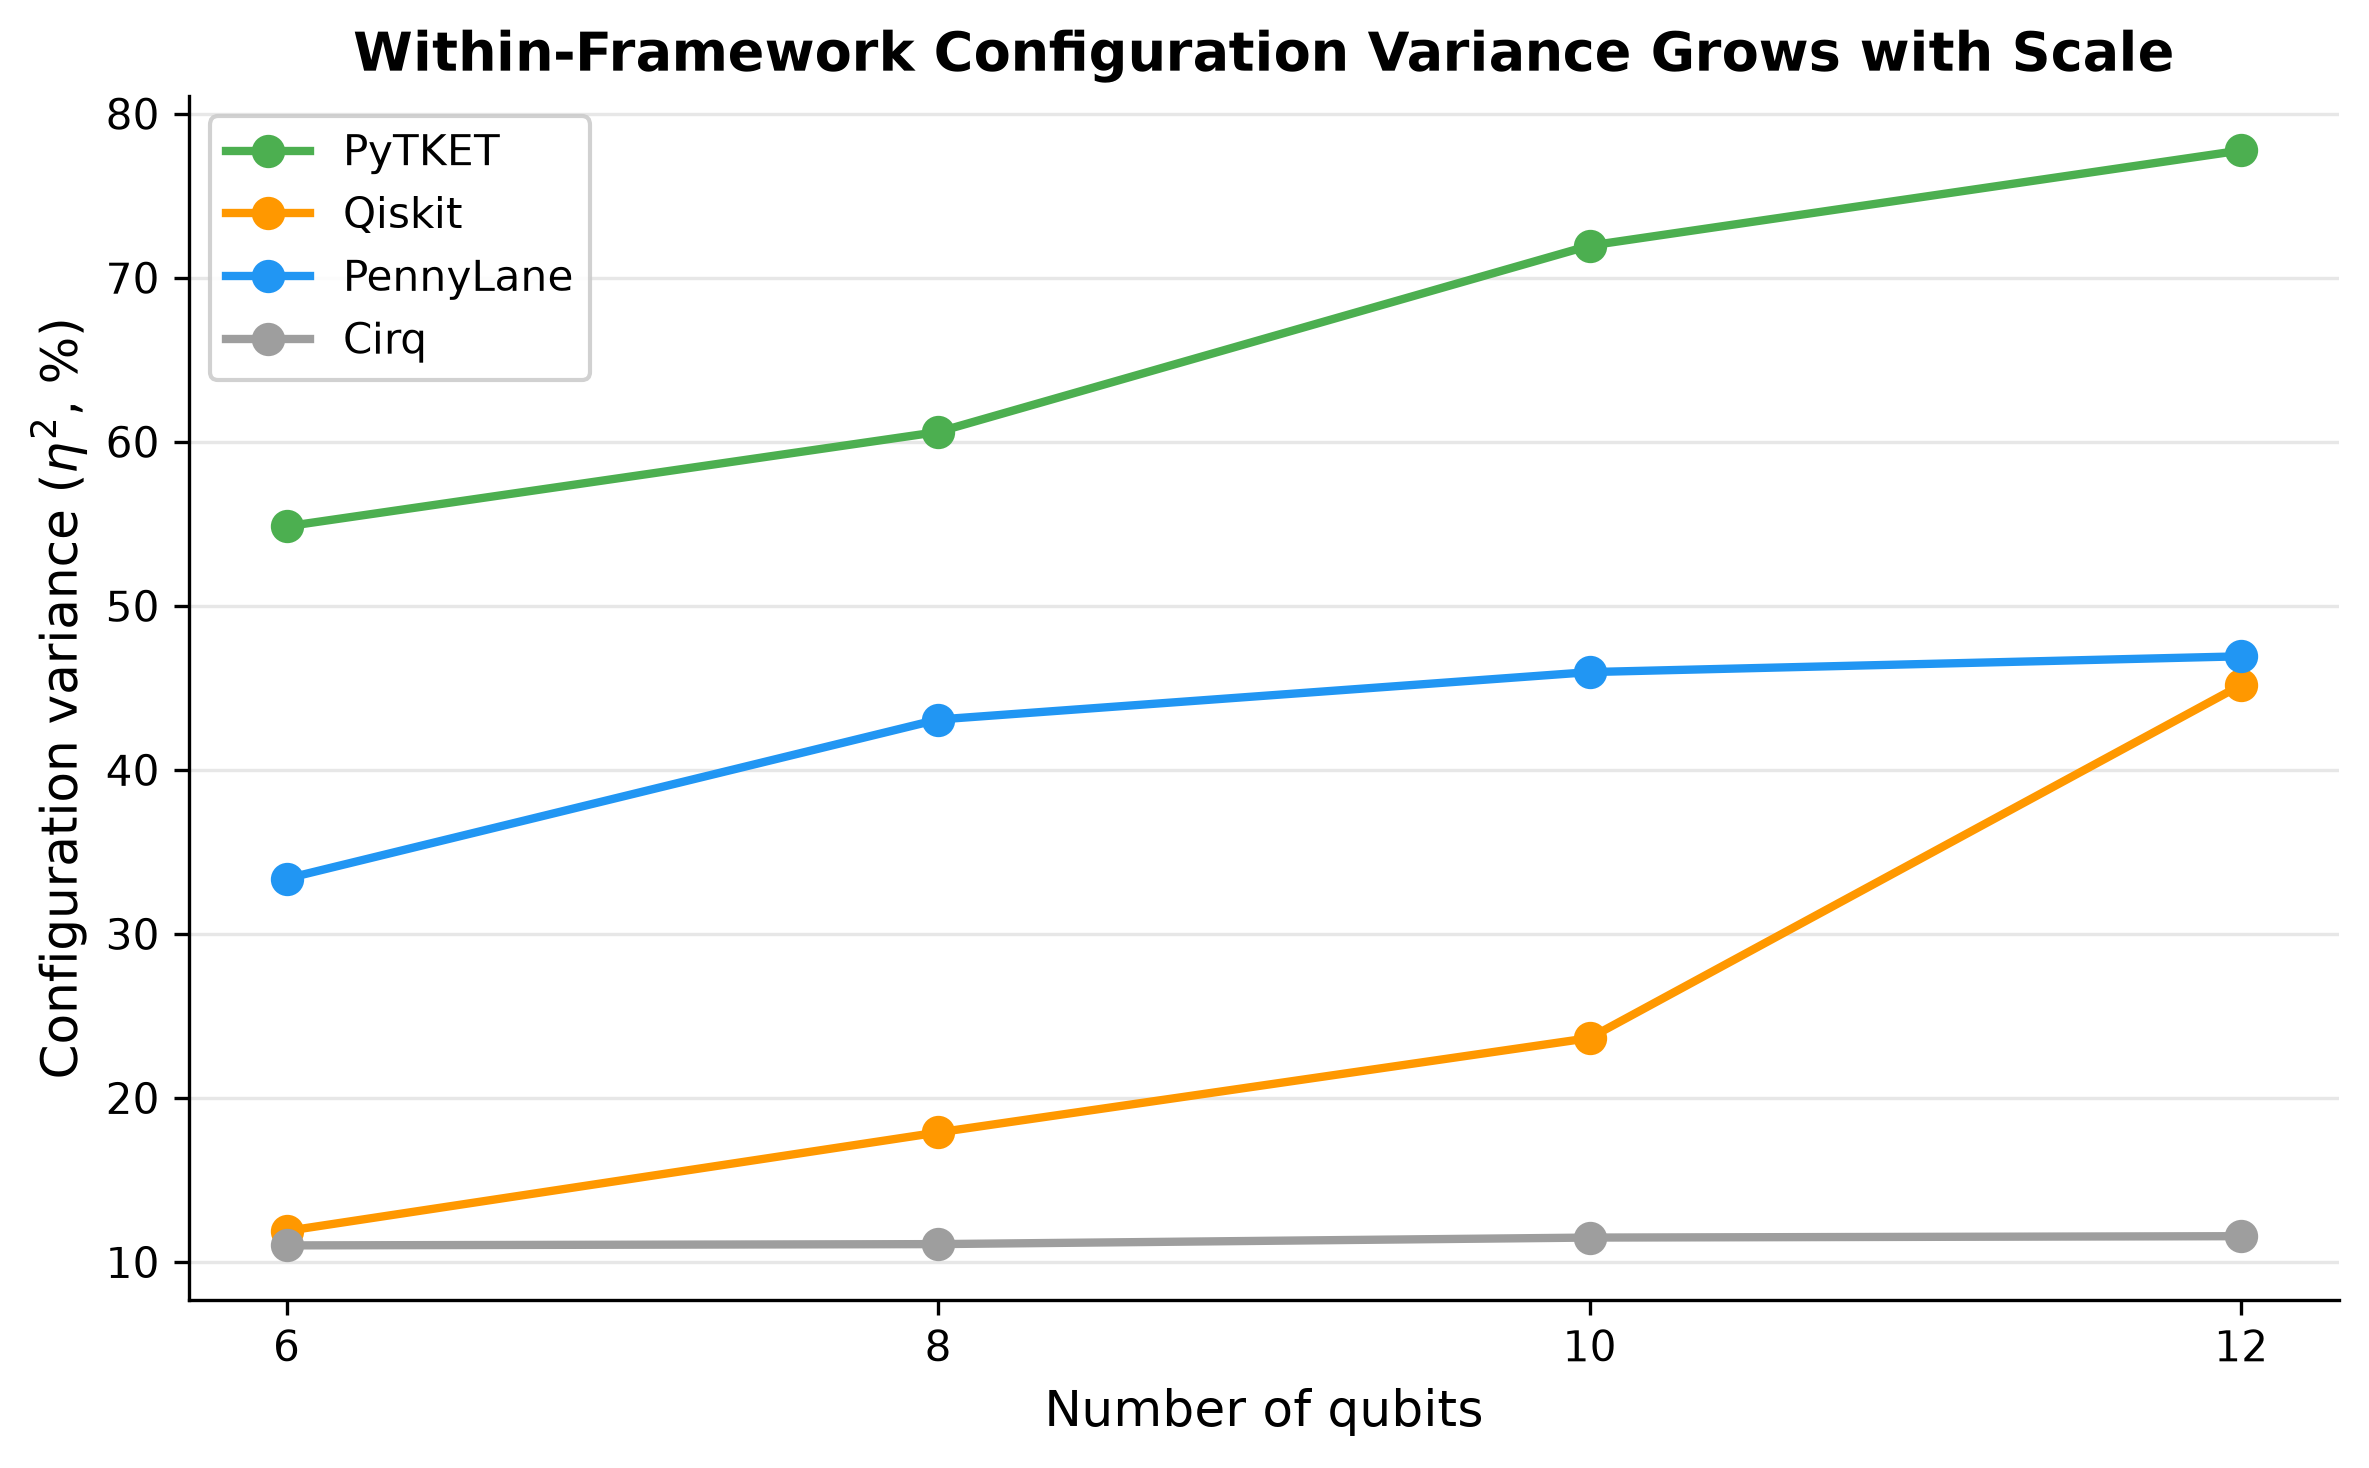
\includegraphics[width=0.85\textwidth]{../figures/fig3_config_variance_growth.png}
\caption{Within-framework configuration variance grows with circuit scale for three of four frameworks. PyTKET's configuration choice explains 78\% of depth variance at 12 qubits. Cirq's small search space (6 configurations) keeps its config variance stable at $\sim$11\%.}
\label{fig:config_variance}
\end{figure}

\subsection{Search value: improvement from representation search}

Table~\ref{tab:search_improvement} summarizes the improvement from representation search: the reduction in depth from the mean configuration to the best configuration within each cell.

\begin{table}[H]
\centering
\caption{Search improvement statistics (best vs.\ mean depth per cell)}
\label{tab:search_improvement}
\begin{tabular}{lc}
\toprule
Statistic & Value \\
\midrule
Cells with data & 96 \\
Mean improvement & 31.2\% \\
Median improvement & 29.0\% \\
Minimum improvement & 0.0\% \\
Maximum improvement & 99.0\% \\
Cells with $>$50\% improvement & 26/96 (27\%) \\
Cells with $>$30\% improvement & 45/96 (47\%) \\
\bottomrule
\end{tabular}
\end{table}

Representation search yields substantial improvements. In 47\% of cells, the best configuration is more than 30\% shallower than the mean. Figure~\ref{fig:search_improvement} shows the distribution.

\begin{figure}[H]
\centering
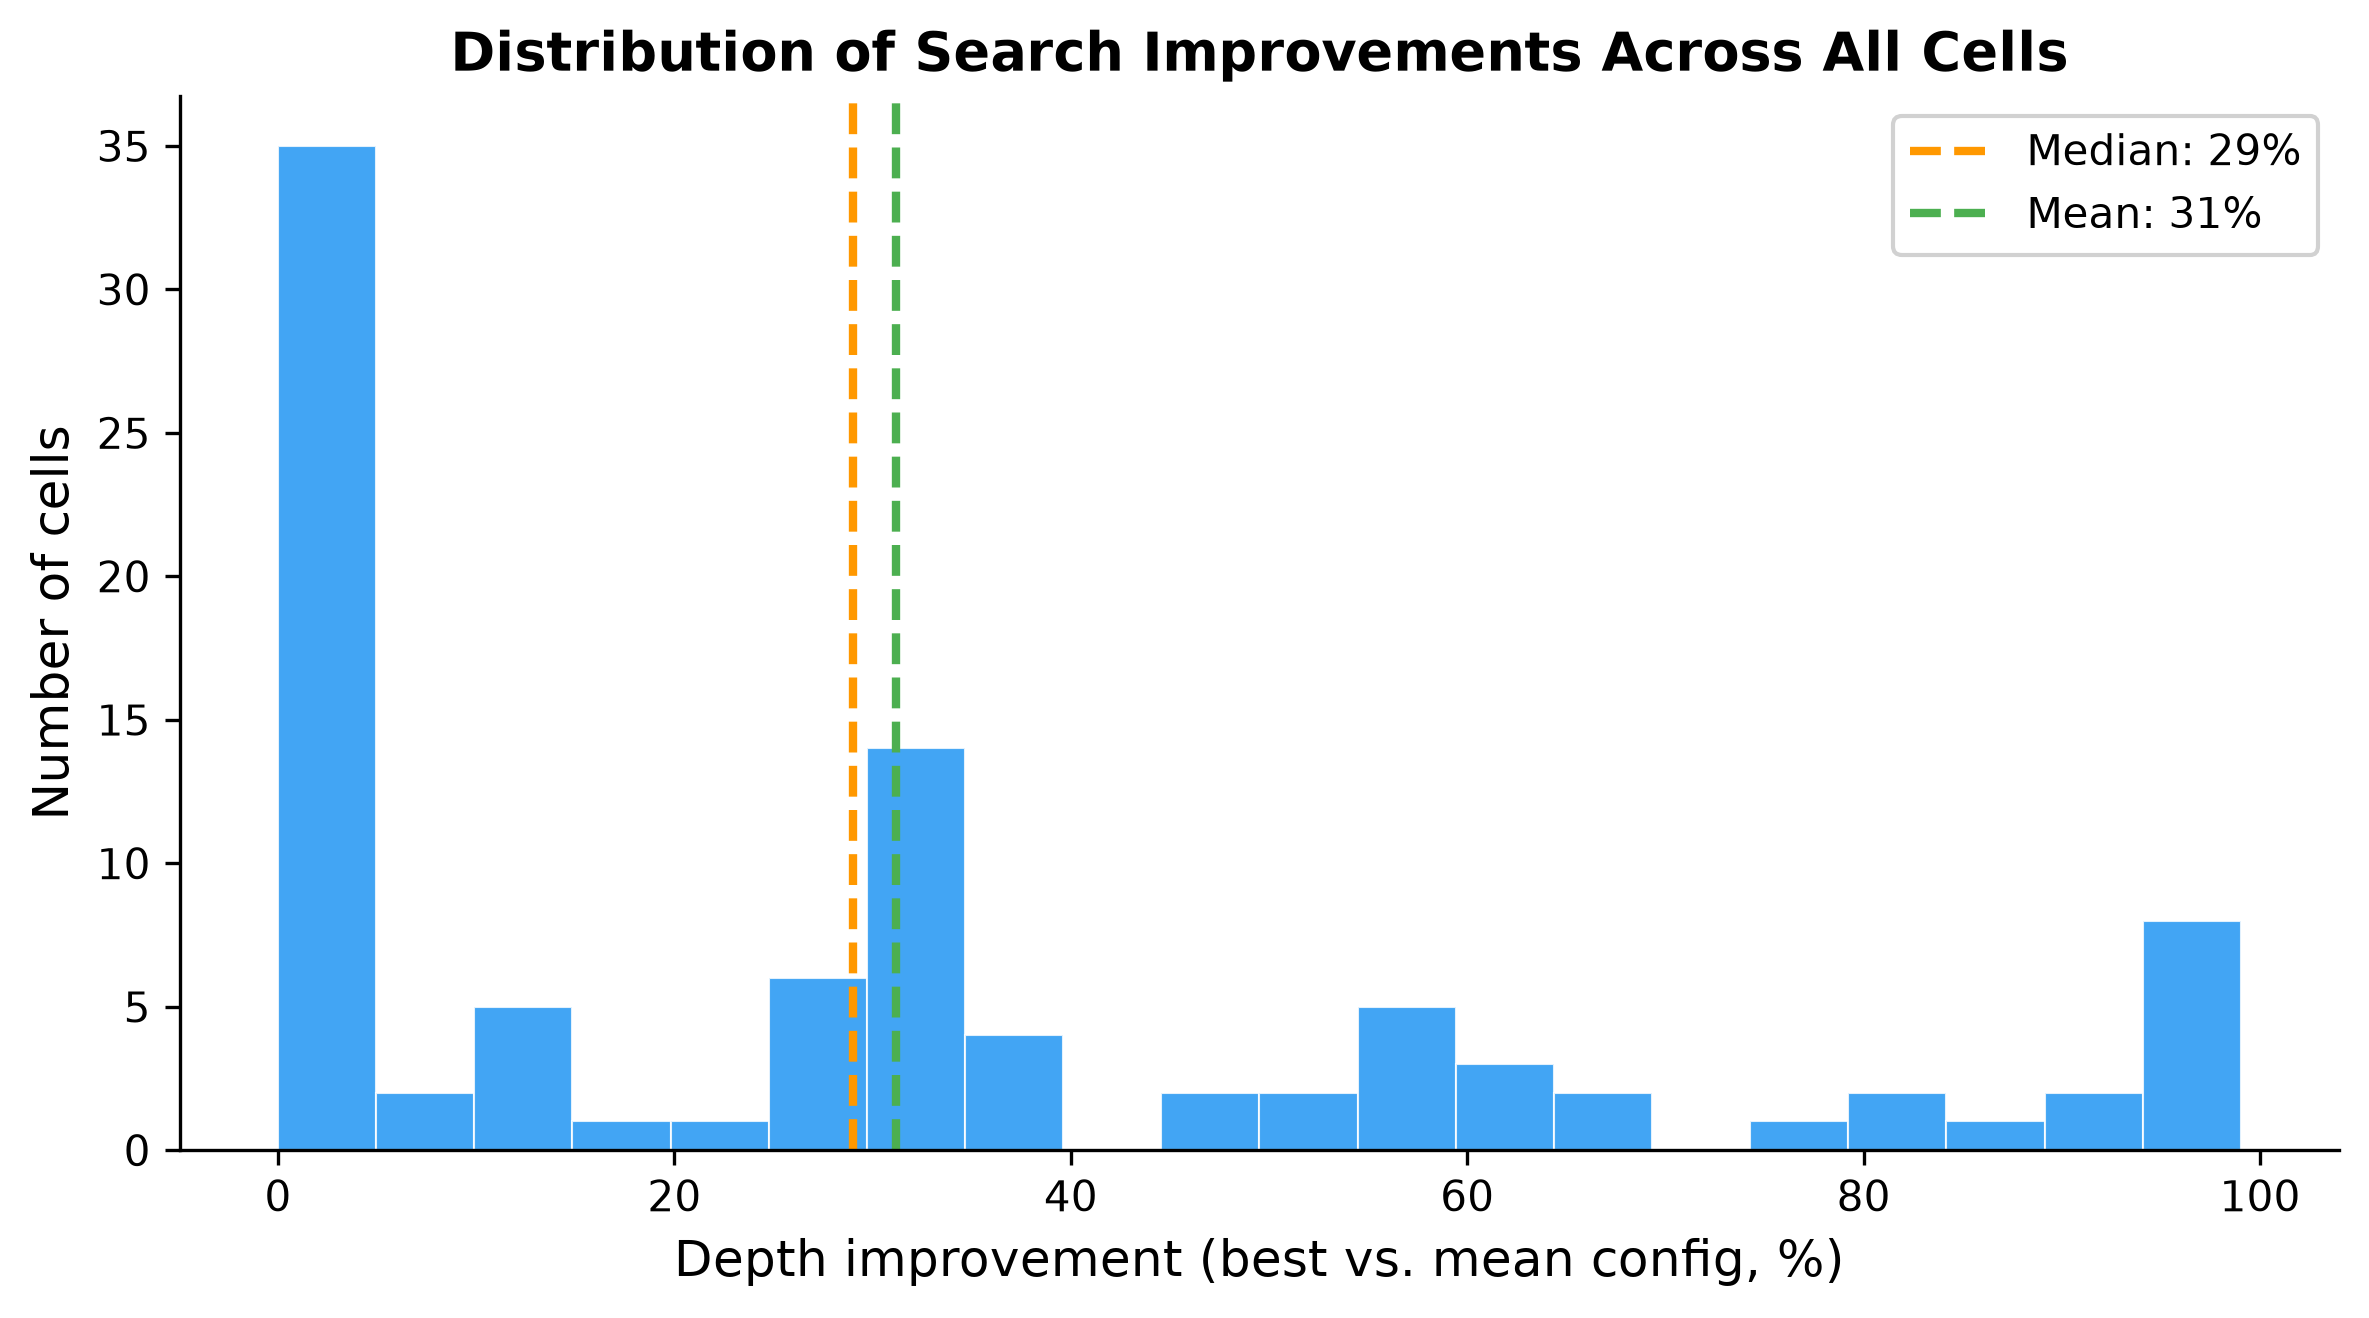
\includegraphics[width=0.85\textwidth]{../figures/fig4_search_improvement.png}
\caption{Distribution of search improvements across all 96 cells. The median improvement is 29\% and the maximum is 99\%. In 47\% of cells, representation search finds a configuration more than 30\% shallower than the mean.}
\label{fig:search_improvement}
\end{figure}

\subsection{Cross-framework comparison}

Table~\ref{tab:best_depth_12q} shows the best achievable depth per algorithm per framework at 12 qubits.

\begin{table}[H]
\centering
\caption{Best depth per algorithm per framework at 12 qubits}
\label{tab:best_depth_12q}
\begin{tabular}{lrrrr}
\toprule
Algorithm & Cirq & PennyLane & PyTKET & Qiskit \\
\midrule
QFT           & 85   & 22  & 24   & 182 \\
Grover        & 6{,}610 & 13  & 7    & 4{,}519 \\
QPE           & 229  & 23  & 24   & 184 \\
GHZ           & 24   & 12  & 13   & 40 \\
BV            & 21   & 13  & 12   & 37 \\
Superposition & 5    & 3   & 3    & 3 \\
\bottomrule
\end{tabular}
\end{table}

The most striking result is Grover at 12 qubits: Cirq produces depth 6{,}610 while PyTKET produces depth 7---a 944$\times$ difference from the same logical circuit. Qiskit produces depth 4{,}519, still 645$\times$ worse than PyTKET. This is entirely attributable to representation choice: different frameworks decompose the multi-controlled Toffoli gate (used in Grover's oracle and diffuser) using fundamentally different strategies, producing wildly different circuit depths.

Figure~\ref{fig:best_depth_12q} visualizes this comparison on a logarithmic scale.

\begin{figure}[H]
\centering
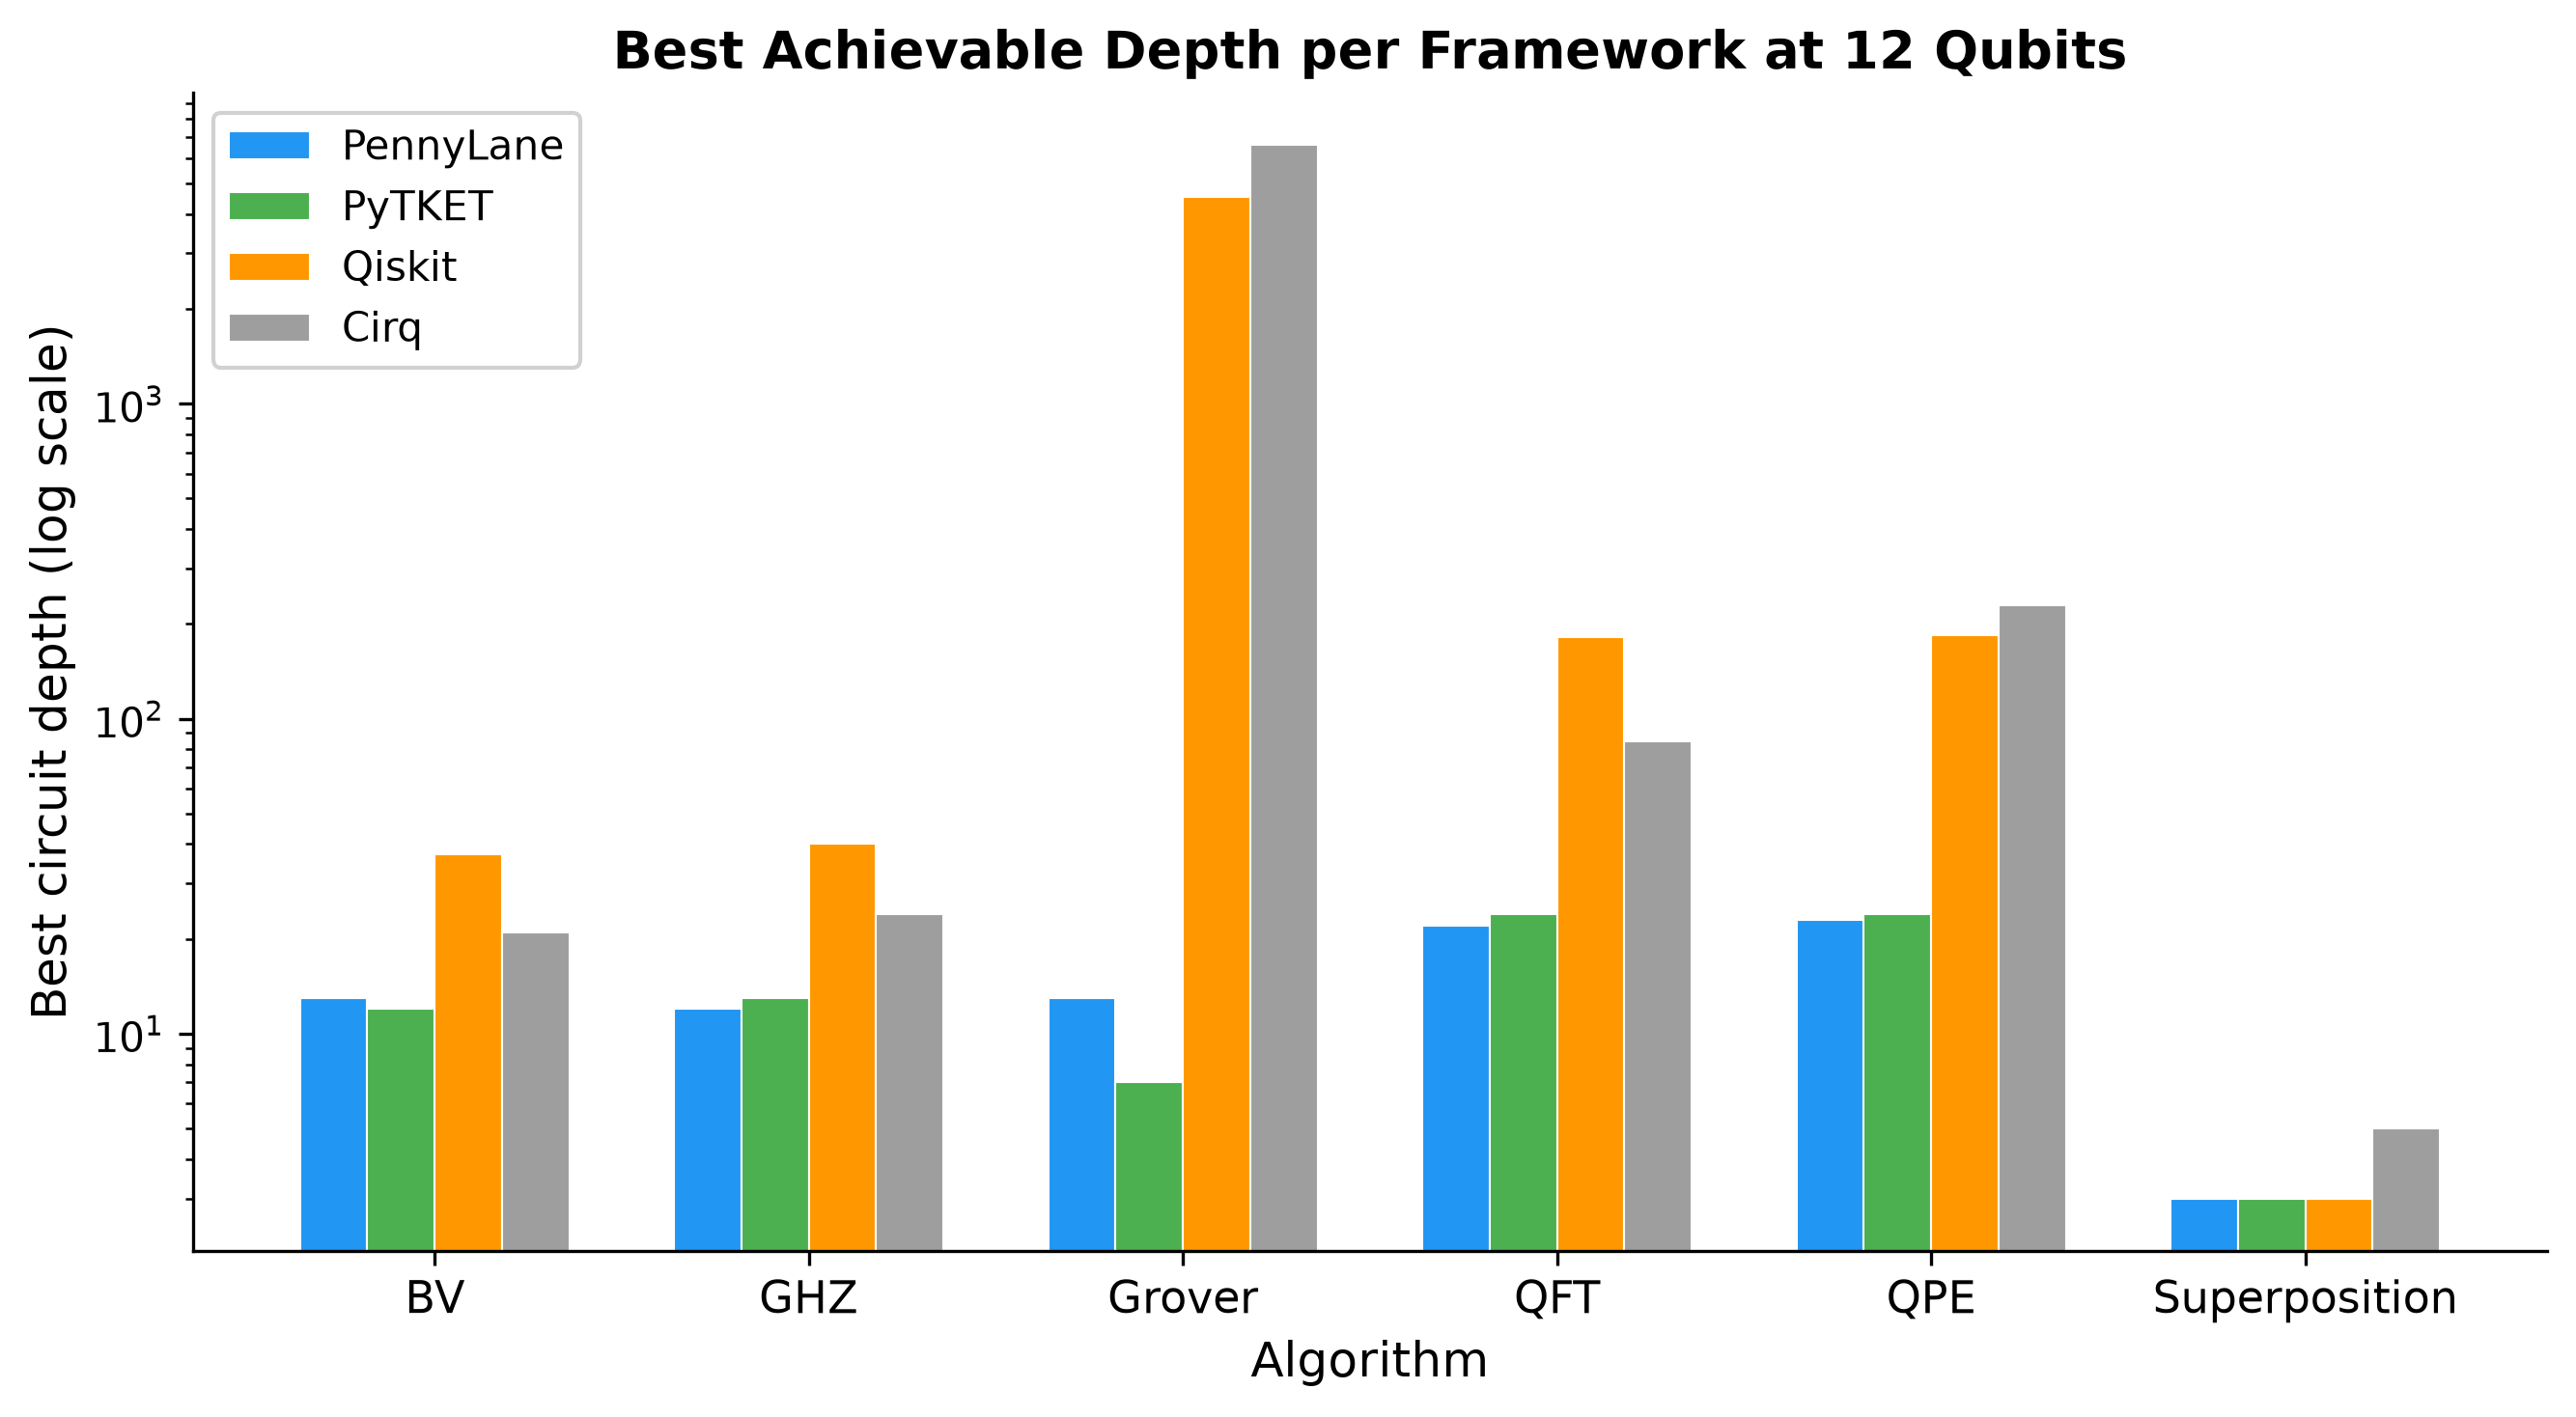
\includegraphics[width=0.9\textwidth]{../figures/fig2_best_depth_12q.png}
\caption{Best achievable depth per framework at 12 qubits (log scale). Grover shows the most extreme variation: PyTKET achieves depth 7 while Cirq produces depth 6{,}610---a 944$\times$ difference from the same logical circuit.}
\label{fig:best_depth_12q}
\end{figure}

\subsection{The Grover case study}

Grover's algorithm provides the most dramatic illustration of the interaction effect. Table~\ref{tab:grover} shows Grover best depth by framework and qubit size.

\begin{table}[H]
\centering
\caption{Grover best depth by framework and qubit size}
\label{tab:grover}
\begin{tabular}{lrrrr}
\toprule
Qubits & Cirq & PennyLane & PyTKET & Qiskit \\
\midrule
6  & 782   & 13 & 7 & 521 \\
8  & 2{,}042 & 13 & 7 & 1{,}149 \\
10 & 4{,}030 & 13 & 7 & 2{,}607 \\
12 & 6{,}610 & 13 & 7 & 4{,}519 \\
\bottomrule
\end{tabular}
\end{table}

PennyLane produces depth 13 for Grover at all scales with zero variance---all configurations yield the same result. PyTKET produces depth 7, even better. Cirq produces depth 6{,}610 at 12 qubits---944$\times$ worse than PyTKET. Qiskit's best is 4{,}519 at 12 qubits---645$\times$ worse than PyTKET.

This case study demonstrates three points:
\begin{enumerate}[noitemsep]
\item The framework choice matters enormously (PyTKET vs.\ Cirq: 944$\times$).
\item The configuration choice within a framework matters (PyTKET mean 724 vs.\ best 7 at 12q).
\item The interaction matters: PyTKET dominates for Grover but not for all algorithms (see QPE, where PyTKET and PennyLane are comparable at depth 24 and 23).
\end{enumerate}

% =============================================================================
% 4. DISCUSSION
% =============================================================================

\section{Discussion}

\subsection{No universal winner}

The interaction effect (32--42\% of variance) is the most practically important finding. It means that selecting a single framework and sticking with it is suboptimal. A researcher compiling QFT should use PennyLane or PyTKET (depth 22--24 at 12q), while a researcher compiling GHZ can use any framework (all produce depth 12--40 at 12q). The optimal framework depends on the algorithm, and no framework is universally best.

This finding has practical implications: quantum software stacks should support multi-framework compilation search, not just single-framework optimization. The WestQuant ecosystem's plugin architecture~\cite{ref12} is designed for exactly this use case.

\subsection{Representation search grows in importance with scale}

The within-framework decomposition (Table~\ref{tab:within_framework}) shows that configuration variance grows with circuit size for three of four frameworks. For PyTKET, configuration explains 55\% of depth variance at 6 qubits but 78\% at 12 qubits. For Qiskit, the growth is from 12\% to 45\%.

This means that at small scales, the algorithm identity is the primary determinant of compilation quality. At larger scales, the configuration choice becomes equally or more important. This trend suggests that representation search will become even more critical as quantum circuits scale to 20+ qubits.

The growing residual term in the two-factor decomposition (from 11\% at 6q to 35\% at 12q) supports this interpretation: at larger scales, within-cell variance (configuration choice) dominates over between-cell variance (algorithm and framework identity).

\subsection{Search spaces are structurally different}

The four frameworks expose fundamentally different representation dimensions (Table~\ref{tab:search_spaces}). Qiskit and PyTKET search compiler configuration space (which passes to apply), but with different pass options. PennyLane searches gate-level transform space (which gate rewrites to apply). Cirq searches gate set and pass count.

This structural difference has two consequences. First, the frameworks are not interchangeable: a configuration that is optimal in Qiskit has no direct analog in PennyLane. Second, the search space size correlates with configuration variance: PyTKET (108 configs, 78\% config variance at 12q) has a much larger search space than Cirq (6 configs, 12\% config variance). Frameworks with larger search spaces offer more optimization room but require more search effort.

Notably, PennyLane's search space (24 configs) is smaller than PyTKET's (108) but its config variance (47\%) is comparable to Qiskit's (45\% at 12q), suggesting that the \textit{nature} of the search dimensions matters as much as their count. PennyLane's gate-level transforms (commute, cancel, merge) are more impactful per-dimension than Qiskit's compiler configuration options.

\subsection{Practical value of representation search}

The search improvement statistics (Table~\ref{tab:search_improvement}) show that representation search is practically valuable. The median improvement of 29\% and the 90th percentile of $\sim$70\% mean that a researcher who runs a representation search rather than accepting the default configuration will typically get a 29\% shallower circuit, and sometimes a 70--99\% shallower one.

At 12 qubits, the improvements are most dramatic for Grover (99\%+ across all frameworks) and QPE (97--99\% across all frameworks). These are not marginal gains---they are the difference between a circuit that fits on a device and one that does not.

\subsection{Implications for ML-guided compilation}

The structured training records produced by the WestQuant search engines~\cite{ref12}, in the WQDF (WestQuant Dataset Format), enable a natural follow-up: training a policy model to predict good representations for unseen circuits. The variance decomposition results suggest that such a model should be framework-specific (since search spaces are structurally different) and scale-aware (since configuration importance grows with circuit size). Cross-framework transfer learning may be challenging because the configuration spaces are not directly comparable.

\subsection{Limitations}

\begin{enumerate}[noitemsep]
\item \textbf{Verification limit:} Exact unitary verification is infeasible beyond 8 qubits due to the $O(4^n)$ memory cost of storing the unitary matrix. At 10--12 qubits, we report compilation metrics without equivalence verification. All frameworks produce valid compilations by construction (the compilation passes preserve equivalence), but we cannot independently verify this at scale.
\item \textbf{Linear topology only:} All experiments use a linear (nearest-neighbor) coupling map. Different topologies (grid, all-to-all, heavy-hex) may produce different variance decompositions. The interaction effect may be larger on more restrictive topologies (where routing matters more) or smaller on less restrictive ones.
\item \textbf{Configuration subset:} We test a subset of each framework's full configuration space (32 of 128 for Qiskit, 32 of 108 for PyTKET). The full grid may reveal additional variance structure.
\item \textbf{Algorithm coverage:} Six algorithms provide a representative but not exhaustive sample. Variational algorithms (VQE, QAOA) with parameterized circuits are not included due to current framework limitations with parameterized circuit conversion.
\item \textbf{Framework versions:} Results are specific to the framework versions tested (Qiskit 2.5.2, PyTKET 2.18.4, PennyLane 0.45.1, Cirq 1.7.0). Newer versions may change the variance structure.
\item \textbf{Cirq Grover timing:} Cirq's Grover compilation is significantly slower than other frameworks (101s per replicate at 12q vs.\ 4s for Qiskit), likely due to the gate set decomposition strategy. This does not affect the depth results but affects practical usability.
\end{enumerate}

% =============================================================================
% 5. CONCLUSION
% =============================================================================

\section{Conclusion}

We have shown that quantum compilation representation is a genuine optimization variable, not a fixed choice. The framework $\times$ algorithm interaction explains 32--42\% of circuit depth variance across 6--12 qubit circuits, meaning no single framework is universally optimal. Within a single framework, configuration choice explains up to 78\% of depth variance at 12 qubits, and this fraction grows with circuit scale. The four frameworks we tested expose structurally different representation search spaces, meaning the optimization landscape is framework-dependent.

Representation search yields a median depth reduction of 29\% and a maximum of 99\% relative to mean configurations. In 47\% of tested cells, the best configuration is more than 30\% shallower than the mean. These are not marginal gains---they are the difference between a compilable and an uncompilable circuit.

These findings motivate a shift in how quantum compilation is approached: from accepting a single framework's default configuration to systematically searching the representation space across frameworks and configurations. The WestQuant open-source ecosystem provides the tooling for this search, and the structured WQDF training records it produces enable future ML-guided approaches to representation selection.

% =============================================================================
% REFERENCES
% =============================================================================

\begin{thebibliography}{99}

\bibitem{ref1} Qiskit contributors. \textit{Qiskit: An open-source framework for quantum computing.} \url{https://qiskit.org}, 2024.

\bibitem{ref2} S.~Sivarajah et al. ``t$|$ket$\rangle$: A retargetable compiler for NISQ devices.'' \textit{Quantum Science and Technology} 6(1):014003, 2020.

\bibitem{ref3} V.~Bergholm et al. ``PennyLane: Automatic differentiation of hybrid quantum-classical computations.'' \textit{arXiv:1811.04968}, 2022.

\bibitem{ref4} Cirq contributors. \textit{Cirq: A Python framework for creating, editing, and invoking Noisy Intermediate Scale Quantum (NISQ) circuits.} \url{https://github.com/quantumlib/Cirq}, 2024.

\bibitem{ref5} T.~Lubinski et al. ``Application-Oriented Performance Benchmarks for Quantum Computing.'' \textit{IEEE Transactions on Quantum Engineering}, vol.~4, pp.~1--32, 2023. arXiv:2110.03137.

\bibitem{ref6} P.~D.~Nation et al. ``Benchmarking the performance of quantum computing software for quantum circuit creation, manipulation and compilation.'' \textit{Nature Computational Science} 5(5):427--435, 2025. doi:10.1038/s43588-025-00792-y.

\bibitem{ref7} Y.~Kharkov et al. ``Arline Benchmarks: Automated Benchmarking Platform for Quantum Compilers.'' arXiv:2202.14025, 2022.

\bibitem{ref8} N.~Quetschlich, L.~Burgholzer, R.~Wille. ``Achieving Pareto-Optimality in Quantum Circuit Compilation via a Multi-Objective Heuristic Optimization Approach.'' In \textit{IEEE International Conference on Quantum Computing and Engineering (QCE)}, 2024. doi:10.1109/QCE60285.2024.10297.

\bibitem{ref9} A.~Rajaei, M.~Houshmand, S.~A.~Hosseini. ``A dynamic programming approach to multi-objective logic synthesis of quantum circuits.'' \textit{Quantum Information Processing} 22:384, 2023. doi:10.1007/s11128-023-04112-z.

\bibitem{ref10} R.~C.~Whaley, A.~Petitet, J.~J.~Dongarra. ``Automated Empirical Optimization of Software and the ATLAS Project.'' \textit{Parallel Computing} 27(1--2):3--35, 2001. doi:10.1016/S0167-8191(00)00087-9.

\bibitem{ref11} S.~Fossati et al. ``Quarl: A Learning-Based Quantum Circuit Optimizer.'' arXiv:2307.10120, 2023.

\bibitem{ref12} D.~Vesterlund. \textit{WestQuant: An open-source ecosystem for quantum representation search.} \url{https://github.com/VesterlundCoder/quantum-representation}, 2025.

\end{thebibliography}

% =============================================================================
% APPENDICES
% =============================================================================

\appendix

\section{Full variance decomposition tables}

\subsection{Circuit depth}

\begin{table}[H]
\centering
\begin{tabular}{cccccc}
\toprule
Qubits & $\eta^2$(algorithm) & $\eta^2$(framework) & $\eta^2$(interaction) & $\eta^2$(residual) & $n$ \\
\midrule
6  & 34.0 & 13.7 & 41.0 & 11.3 & 1{,}152 \\
8  & 31.2 & 12.6 & 42.5 & 13.7 & 1{,}152 \\
10 & 28.6 & 12.6 & 41.6 & 17.2 & 1{,}152 \\
12 & 23.4 & 10.5 & 31.6 & 34.5 & 1{,}152 \\
\bottomrule
\end{tabular}
\end{table}

\subsection{Two-qubit gate count}

\begin{table}[H]
\centering
\begin{tabular}{cccccc}
\toprule
Qubits & $\eta^2$(algorithm) & $\eta^2$(framework) & $\eta^2$(interaction) & $\eta^2$(residual) & $n$ \\
\midrule
6  & 66.5 & 16.9 & 19.5 & 0.0 & 1{,}041 \\
8  & 61.7 & 16.7 & 21.5 & 0.1 & 1{,}041 \\
10 & 58.5 & 17.2 & 22.7 & 1.6 & 1{,}041 \\
12 & 49.9 & 15.4 & 20.3 & 14.4 & 1{,}041 \\
\bottomrule
\end{tabular}
\end{table}

\subsection{Within-framework configuration variance}

\begin{table}[H]
\centering
\begin{tabular}{lcccc}
\toprule
Framework & 6q & 8q & 10q & 12q \\
\midrule
PyTKET    & 54.8 & 60.6 & 72.0 & 77.8 \\
Qiskit    & 11.9 & 17.9 & 23.7 & 45.2 \\
PennyLane & 33.4 & 43.1 & 46.0 & 46.9 \\
Cirq      & 11.0 & 11.1 & 11.5 & 11.6 \\
\bottomrule
\end{tabular}
\end{table}

\section{Best depth per algorithm per framework}

\subsection{6 qubits}

\begin{table}[H]
\centering
\begin{tabular}{lrrrr}
\toprule
Algorithm & Cirq & PennyLane & PyTKET & Qiskit \\
\midrule
BV            & 9   & 7  & 6  & 21 \\
GHZ           & 12  & 6  & 7  & 18 \\
Grover        & 782 & 13 & 7  & 521 \\
QFT           & 37  & 10 & 12 & 66 \\
QPE           & 49  & 11 & 12 & 61 \\
Superposition & 5   & 3  & 3  & 3 \\
\bottomrule
\end{tabular}
\end{table}

\subsection{8 qubits}

\begin{table}[H]
\centering
\begin{tabular}{lrrrr}
\toprule
Algorithm & Cirq & PennyLane & PyTKET & Qiskit \\
\midrule
BV            & 13    & 9  & 8  & 28 \\
GHZ           & 16    & 8  & 9  & 24 \\
Grover        & 2{,}042 & 13 & 7  & 1{,}149 \\
QFT           & 53    & 14 & 16 & 106 \\
QPE           & 93    & 15 & 16 & 109 \\
Superposition & 5     & 3  & 3  & 3 \\
\bottomrule
\end{tabular}
\end{table}

\subsection{10 qubits}

\begin{table}[H]
\centering
\begin{tabular}{lrrrr}
\toprule
Algorithm & Cirq & PennyLane & PyTKET & Qiskit \\
\midrule
BV            & 17    & 11 & 10 & 29 \\
GHZ           & 20    & 10 & 11 & 32 \\
Grover        & 4{,}030 & 13 & 7  & 2{,}607 \\
QFT           & 69    & 18 & 20 & 155 \\
QPE           & 153   & 19 & 20 & 141 \\
Superposition & 5     & 3  & 3  & 3 \\
\bottomrule
\end{tabular}
\end{table}

\subsection{12 qubits}

\begin{table}[H]
\centering
\begin{tabular}{lrrrr}
\toprule
Algorithm & Cirq & PennyLane & PyTKET & Qiskit \\
\midrule
BV            & 21    & 13 & 12 & 37 \\
GHZ           & 24    & 12 & 13 & 40 \\
Grover        & 6{,}610 & 13 & 7  & 4{,}519 \\
QFT           & 85    & 22 & 24 & 182 \\
QPE           & 229   & 23 & 24 & 184 \\
Superposition & 5     & 3  & 3  & 3 \\
\bottomrule
\end{tabular}
\end{table}

% =============================================================================
% REPRODUCIBILITY
% =============================================================================

\section{Reproducibility}

All data, code, and artifacts for this paper are available at:

\begin{center}
\url{https://github.com/VesterlundCoder/quantum-representation}
\end{center}

The repository contains:
\begin{itemize}[noitemsep]
\item \texttt{data/} --- the full dataset of 4{,}608 observations (\texttt{scale\_observations\_v2.json})
\item \texttt{figures/} --- all generated figures (PNG, 300 DPI)
\item \texttt{manuscript/} --- LaTeX source for this paper
\item \texttt{code/} --- experiment script and figure-generation scripts
\end{itemize}

All numbers and percentages in the manuscript are derived programmatically from the dataset. The experiment can be reproduced by running:
\begin{verbatim}
pip install westquant-core==0.2.0a3 westquant-qiskit==0.1.0a4 \
    westquant-pytket==0.1.0a2 westquant-pennylane==0.1.0a1 \
    westquant-bridges==0.1.0a2 westquant==0.1.0a2
python code/scale_experiment_v2.py
python code/generate_figures.py
\end{verbatim}

% =============================================================================
% DECLARATION OF COMPETING INTERESTS
% =============================================================================

\section*{Declaration of Competing Interests}

The author declares no competing interests. This research received no external funding. The author has no financial or personal relationships with any of the organizations or products discussed in this work that could inappropriately influence the work presented.

% =============================================================================
% AI USE DISCLOSURE
% =============================================================================

\section*{AI Use Disclosure}

Generative AI tools (Claude/Anthropic and ChatGPT/OpenAI) were used during the preparation of this manuscript for the following purposes: generating figures and visualizations, drafting and editing prose, formatting the LaTeX manuscript, and assisting with literature search and screening. The research idea, research questions, taxonomy design, formal mathematical framework, classification of all papers, interpretation of findings, and all scientific judgments are solely the work of the author. Every AI-generated figure, table, and text passage has been reviewed, verified, and corrected by the author. The author takes full responsibility for the accuracy and integrity of all content in this manuscript.

\end{document}
